\documentclass[10pt,a4paper]{article}
\usepackage[margin=1.4cm]{geometry}
\usepackage{helvet}\renewcommand{\familydefault}{\sfdefault}
\usepackage{graphicx,booktabs,xcolor,fancyhdr,multicol,float}
\definecolor{bigorange}{RGB}{255,130,0}
\definecolor{biggrey}{RGB}{60,60,60}
\pagestyle{fancy}\fancyhf{}
\lhead{\textbf{\color{bigorange}Banco BIG} \color{biggrey}| Rates Research}
\rhead{\color{biggrey}\today}
\renewcommand{\headrulewidth}{1pt}
\setlength{\parindent}{0pt}\setlength{\parskip}{4pt}
\begin{document}
\begin{center}
{\Large\textbf{\color{biggrey}US Treasury Positioning \& the 10Y Yield}}\\[2pt]
{\color{bigorange}\rule{\textwidth}{2pt}}\\[2pt]
{\small A CFTC-positioning crowding study + a dynamic US10Y ARIMA forecaster — free-data, reproducible.}
\end{center}

\textbf{\color{bigorange}1. What positioning measures \& where we are}\\
We convert CFTC Traders-in-Financial-Futures net positions (TU/FV/TY/TN/US/UB) into DV01, aggregate by
trader type, z-score, and reduce to a PCA composite crowding index (+ = crowded net \emph{long} duration).
As of \textbf{2026-07-14} the composite is \textbf{+2.49} — a multi-year \emph{crowded-long}
extreme, driven by asset managers (long the long end) with dealers mirror-short.

\begin{figure}[H]\centering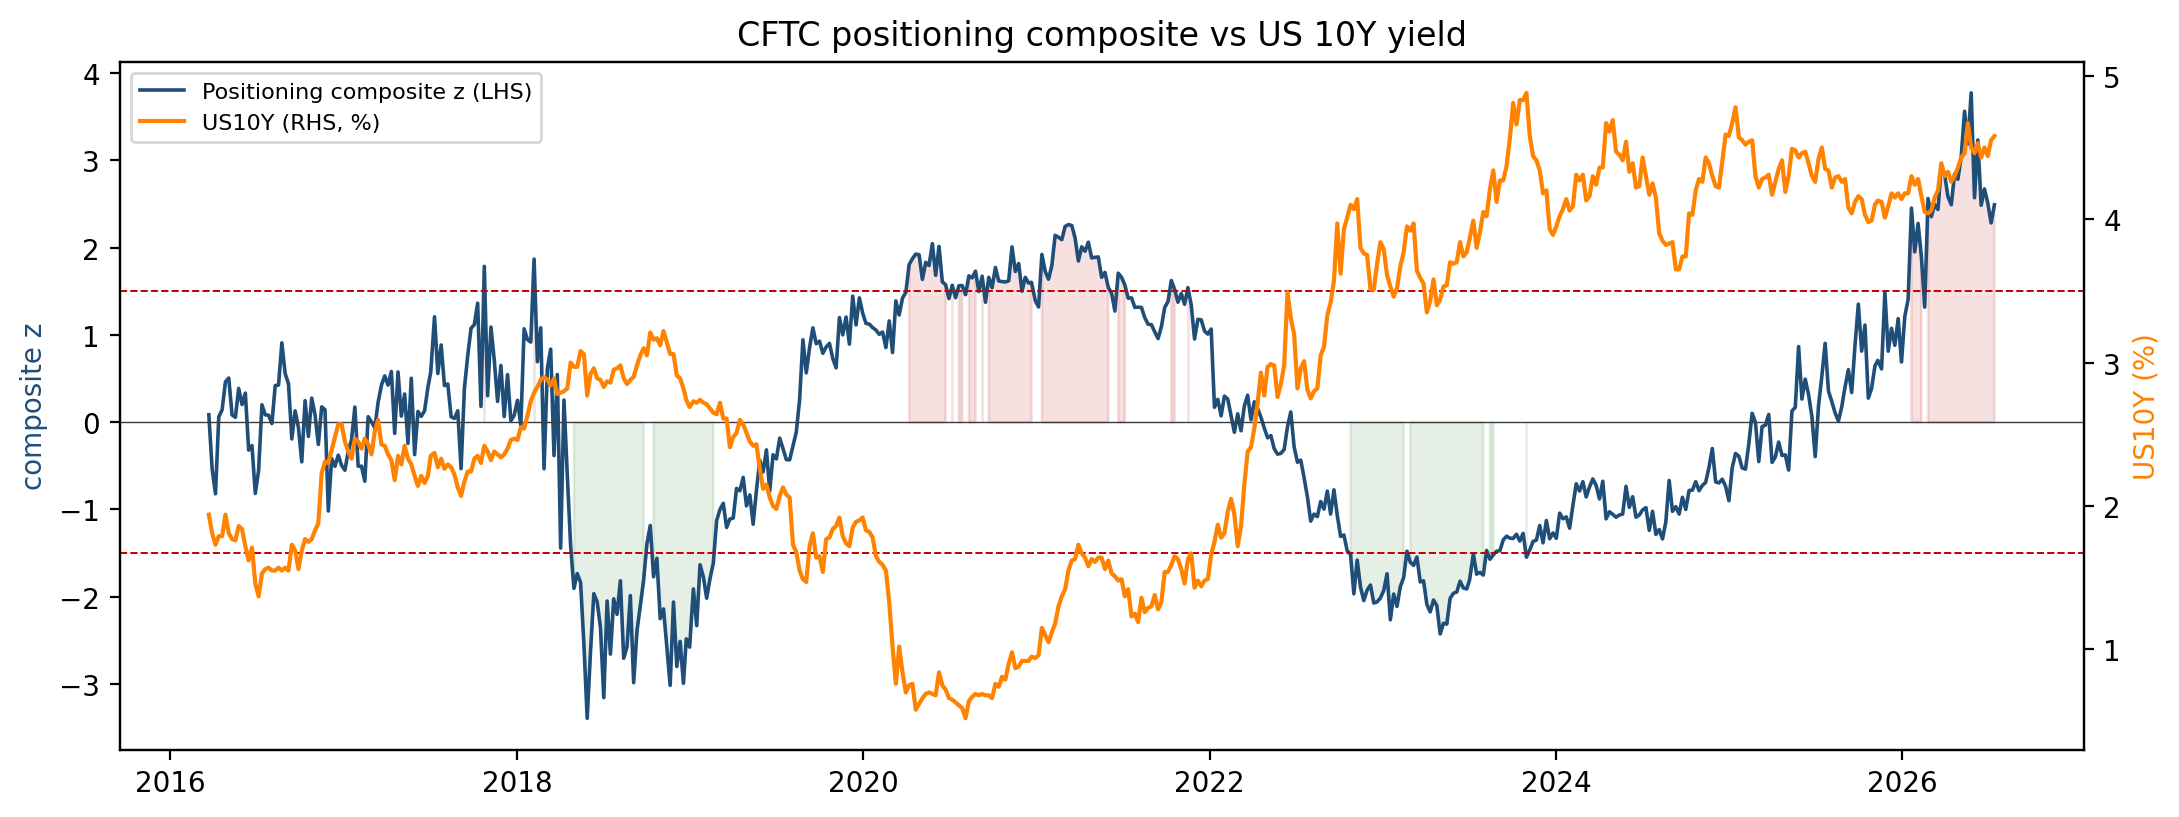
\includegraphics[width=0.98\textwidth]{fig_composite_vs_yield.png}\end{figure}

\textbf{\color{bigorange}2. Does crowded positioning precede higher yields? (the honest answer)}\\
Directionally \emph{yes, weakly}: at crowded-long extremes ($z>1.5$) the 10Y rose over the next
4/8/13/26w with probability 0.53/0.63/0.66/0.74
(vs unconditional 0.51/0.56/0.57/0.57),
mean $\Delta y$ +8bp (8w) rising to +33bp (26w).
\textbf{But it is not statistically robust}: 95\% bootstrap CIs include 0.5 at every horizon
(e.g.\ 13w [0.38, 0.91]), Granger causality is insignificant (min p $\approx$ 0.80), and forward-return
regressions are weak (13w $t=+0.66$, $R^2=0.005$;
26w $t=+1.12$). The effect is \textbf{asymmetric} — fading crowded
\emph{longs} works, fading crowded \emph{shorts} does not — and rests on few independent episodes.

\begin{multicols}{2}
\begin{figure}[H]\centering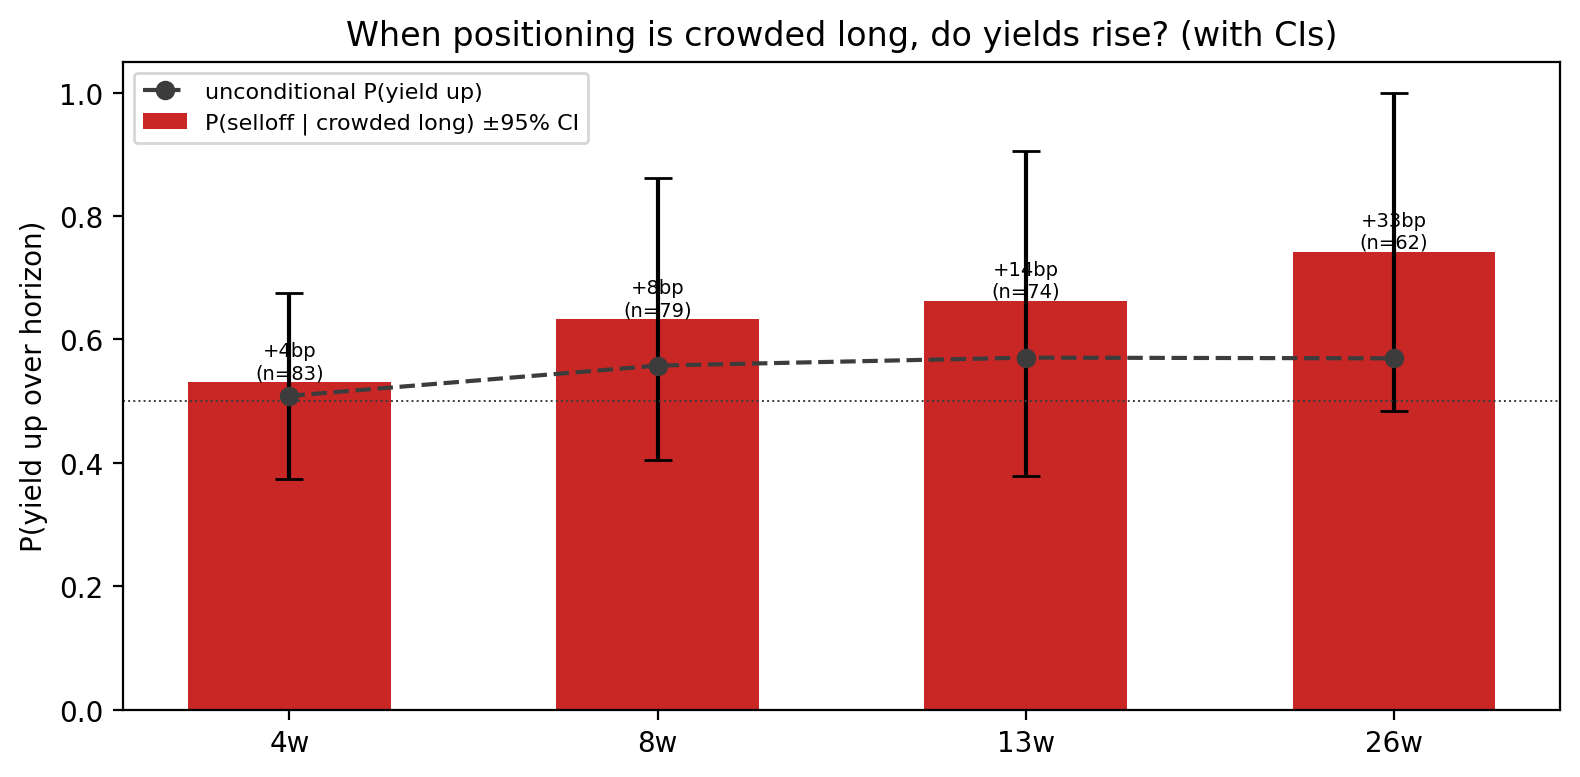
\includegraphics[width=\linewidth]{fig_conditional.png}\end{figure}
\begin{figure}[H]\centering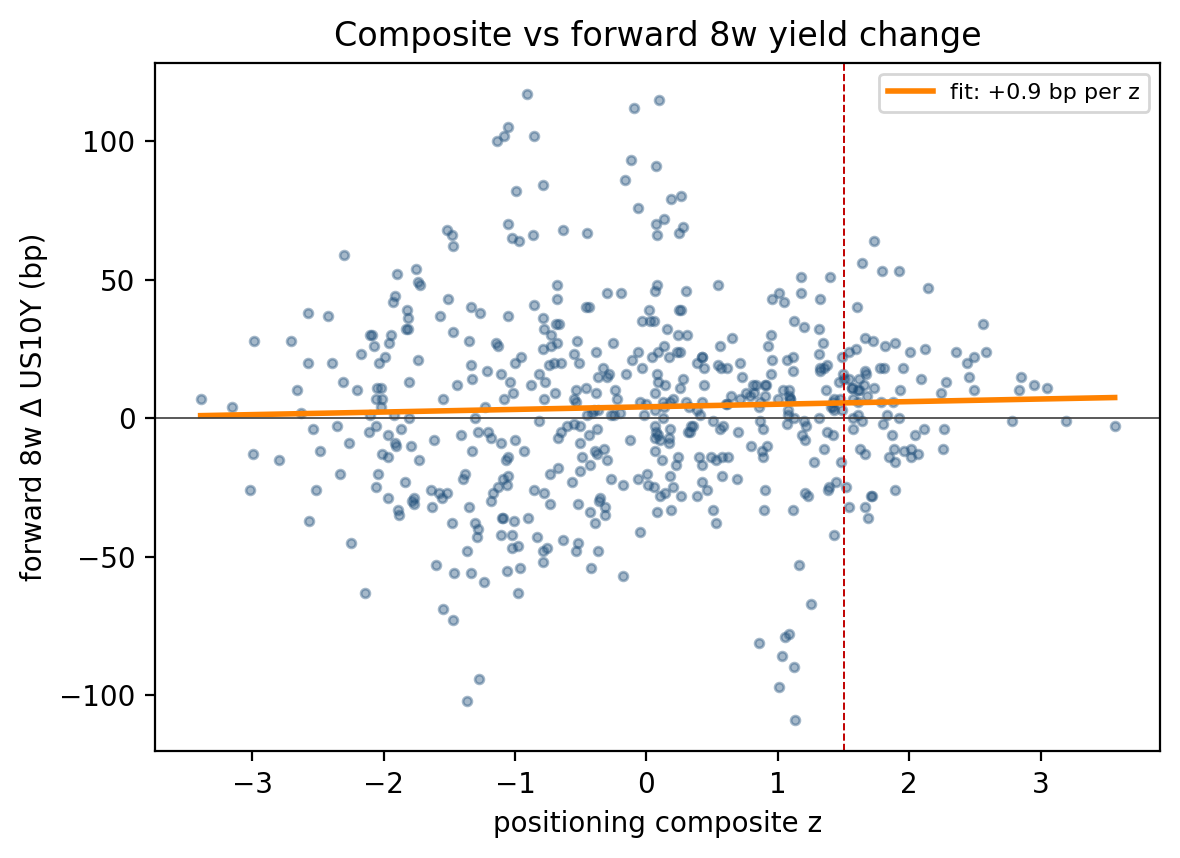
\includegraphics[width=\linewidth]{fig_scatter.png}\end{figure}
\end{multicols}

\textbf{\color{bigorange}3. Dynamic US10Y forecast — simple ARIMA(0, 1, 2)}\\
DGS10 is I(1) (ADF level p=0.32, diff p$<$0.01). A recursive walk-forward
ARIMA(0, 1, 2) gives one-step OOS RMSE \textbf{0.049} vs a random walk
0.049 (ratio 0.999; Diebold–Mariano p=0.62)
— i.e.\ \textbf{statistically indistinguishable from a random walk}, as expected for yields. Adding the
positioning composite as an exogenous regressor (ARIMAX, weekly) does \textbf{not} help out-of-sample
(RMSE ratio 0.999, DM p=0.80). Latest
level 4.63\%; 21-day point forecast 4.63\% (essentially flat).

\begin{figure}[H]\centering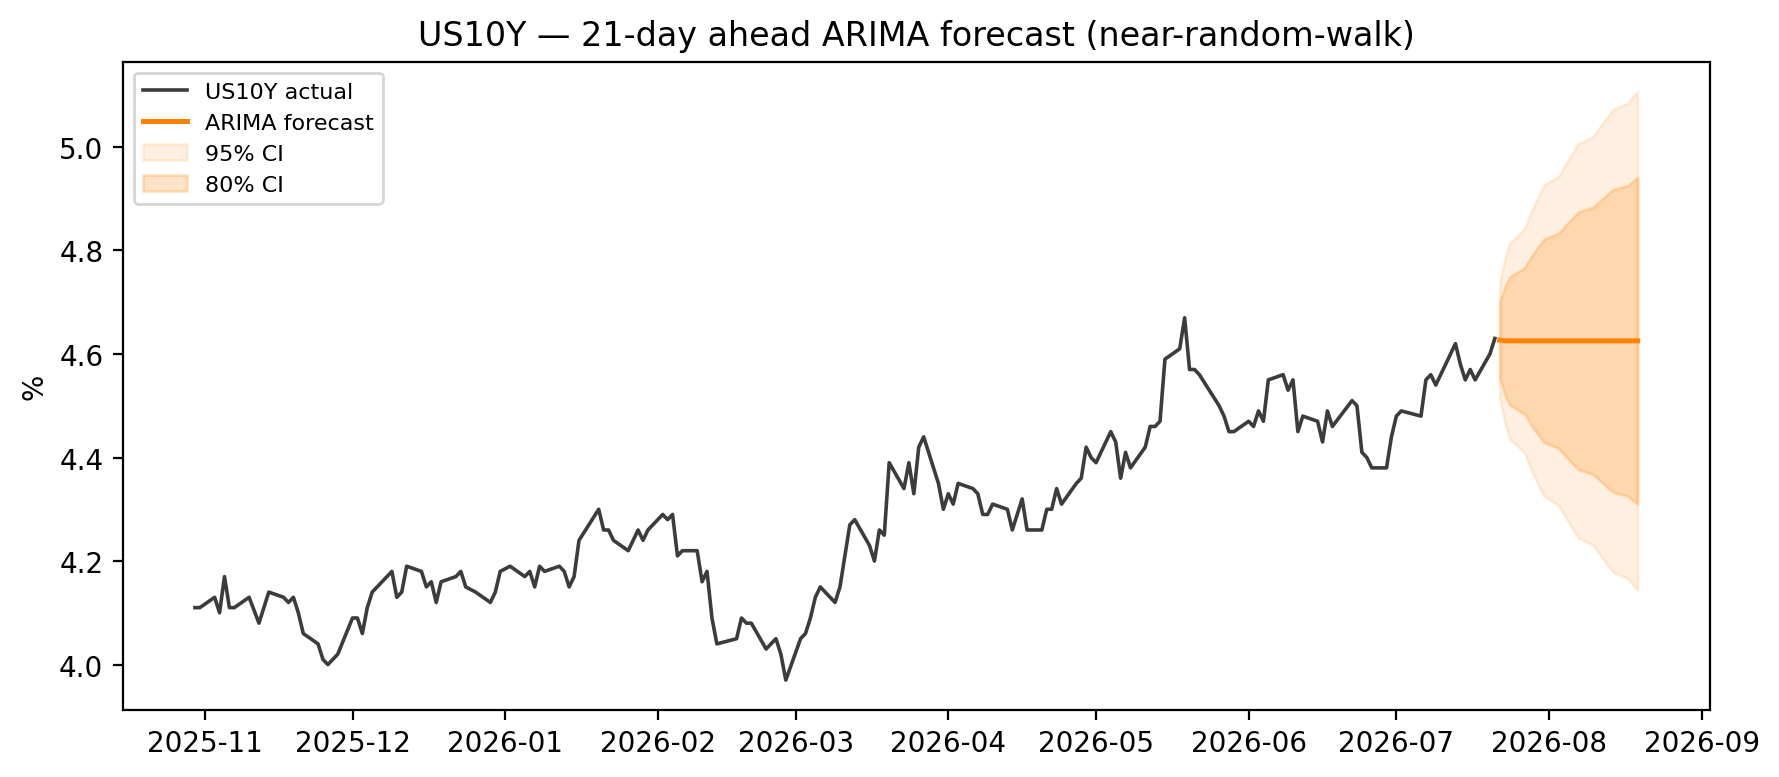
\includegraphics[width=0.98\textwidth]{fig_arima_live.png}\end{figure}

\textbf{\color{bigorange}Bottom line}\\
Positioning is a strong \emph{descriptive} crowding gauge and currently flags a stretched long-duration
market whose modest historical tendency is toward higher yields over 1--6 months — but the predictive
edge is weak and not statistically significant, and neither ARIMA nor positioning beats a random walk for
point-forecasting the 10Y. Use positioning for context and risk framing, not as a standalone yield forecast.

\vspace{4pt}{\footnotesize\color{biggrey}Sources: CFTC TFF (gpe5-46if), FRED DGS10/DGS2. Causal
(publication-lagged) composite; block-bootstrap CIs; expanding-window OOS. Reproduce:
\texttt{python -m rates\_study.run --report}.}
\end{document}
